%%%%%%%%%%%%%%%%%%%%%%%%%%%%%%%%%%%%%%%%%
% Short Sectioned Assignment
% LaTeX Template
% Version 1.0 (5/5/12)
%
% This template has been downloaded from:
% http://www.LaTeXTemplates.com
%
% Original author:
% Frits Wenneker (http://www.howtotex.com)
%
% License:
% CC BY-NC-SA 3.0 (http://creativecommons.org/licenses/by-nc-sa/3.0/)
%
%%%%%%%%%%%%%%%%%%%%%%%%%%%%%%%%%%%%%%%%%

%----------------------------------------------------------------------------------------
%	PACKAGES AND OTHER DOCUMENT CONFIGURATIONS
%----------------------------------------------------------------------------------------

\documentclass[paper=a4, fontsize=11pt]{scrartcl} % A4 paper and 11pt font size

\usepackage{tikz}
\usepackage[T1]{fontenc} % Use 8-bit encoding that has 256 glyphs
\usepackage{float}
%\usepackage{fourier} % Use the Adobe Utopia font for the document - comment this line to return to the LaTeX default


\usepackage[american]{babel} % English language/hyphenation
\usepackage{amsmath,amsfonts,amsthm} % Math packages
\usepackage{bm}

\usepackage{csquotes}
\usepackage[style=apa,sortcites=true,sorting=nyt,backend=biber]{biblatex} %bibliography package
\DeclareLanguageMapping{american}{american-apa}
\nocite{*}

\usepackage{sectsty} % Allows customizing section commands
\allsectionsfont{\centering \normalfont\scshape} % Make all sections centered, the default font and small caps

\usepackage{fancyhdr} % Custom headers and footers
\usepackage{outlines}
\usepackage{enumitem}

\pagestyle{fancyplain} % Makes all pages in the document conform to the custom headers and footers
\fancyhead{} % No page header - if you want one, create it in the same way as the footers below
\fancyfoot[L]{} % Empty left footer
\fancyfoot[C]{} % Empty center footer
\fancyfoot[R]{\thepage} % Page numbering for right footer
\renewcommand{\headrulewidth}{0pt} % Remove header underlines
\renewcommand{\footrulewidth}{0pt} % Remove footer underlines
\setlength{\headheight}{13.6pt} % Customize the height of the header

\numberwithin{equation}{section} % Number equations within sections (i.e. 1.1, 1.2, 2.1, 2.2 instead of 1, 2, 3, 4)
\numberwithin{figure}{section} % Number figures within sections (i.e. 1.1, 1.2, 2.1, 2.2 instead of 1, 2, 3, 4)
\numberwithin{table}{section} % Number tables within sections (i.e. 1.1, 1.2, 2.1, 2.2 instead of 1, 2, 3, 4)

\setlength\parindent{0pt} % Removes all indentation from paragraphs - comment this line for an assignment with lots of text

\bibliography{biblio}
%----------------------------------------------------------------------------------------
%	TITLE SECTION
%----------------------------------------------------------------------------------------

\newcommand{\horrule}[1]{\rule{\linewidth}{#1}} % Create horizontal rule command with 1 argument of height

\title{	
\normalfont \normalsize 
\textsc{Math 460} \\ [25pt] % Your university, school and/or department name(s)
\horrule{0.5pt} \\[0.4cm] % Thin top horizontal rule
\huge Golay Codes\\ % The assignment title
\horrule{2pt} \\[0.5cm] % Thick bottom horizontal rule
}

\author{Dean Bisogno} % Your name

\date{\normalsize\today} % Today's date or a custom date
\newtheoremstyle{break}
  {\topsep}{\topsep}%
  {\itshape}{}%
  {\bfseries}{.}%
  {\newline}{}%
\theoremstyle{break}
\newtheorem{lem}{Lemma}
\newtheorem{defn}{Definition}
\newtheorem{thm}{Theorem}
\newtheorem{cor}{Corollary}
\newtheorem{prop}{Proposition}
\newtheorem{ex}{Example}
\renewcommand\qedsymbol{//}
\newtheorem{lma}{Lemma}
\setenumerate[1]{label=\Roman*.}
\setenumerate[2]{label=\Alph*.}
\setenumerate[3]{label=\roman*.}
\setenumerate[4]{label=\alph*.}

\usepackage{listings}
\usepackage{color}

\definecolor{dkgreen}{rgb}{0,0.6,0}
\definecolor{gray}{rgb}{0.5,0.5,0.5}
\definecolor{mauve}{rgb}{0.58,0,0.82}

\lstset{frame=tb,
  language=Matlab,
  aboveskip=3mm,
  belowskip=3mm,
  showstringspaces=false,
  columns=flexible,
  basicstyle={\small\ttfamily},
  numbers=none,
  numberstyle=\tiny\color{gray},
  keywordstyle=\color{blue},
  commentstyle=\color{dkgreen},
  stringstyle=\color{mauve},
  breaklines=true,
  breakatwhitespace=true,
  tabsize=3
}

\begin{document}
\maketitle % Print the title

\section{History and Constructions}

The Golay code developed by Marcel Golay in 1949 has had significant impact on the advancement of coding theory, the classification of simple finite groups, and communication systems. Golay's 1949 article ``Notes on Digital Coding'' appeared in the June edition of the Proceedings of the IRE [\cite{golay}]. In ``Notes on Digital Coding'' Golay presented a generalization of the Hamming(7,4,3) code which he had read about in Shannon's 1948 paper. After generalizing the perfect, single error-correcting codes, Golay then justifies the existence of two codes which can correct multiple errors, the perfect binary Golay $[23,12,11]_2$ code $\mathcal{G}_{23}$, and the ternary Golay $[11,6,5]_3$ code $\mathcal{G}_{11}$. At the bottom of the article Golay supplied generator matrices for his codes, but lacked any explanation of their construction. Golay would provide explanation of his matrices' construction in 1954. Though brief and without significant justification, Berlekamp called the article ``the best single published page'' and Zaremba once told Golay that he had ``said more in half a page than others have said in twenty pages'' [\cite{thompson}]. The remainder of this section will focus on constructions of $\mathcal{G}_{23}$, $\mathcal{G}_{24}$, and some interesting properties they satisfy. With these constructions and their properties in hand, we will then be able to motivate the study of the Golay codes as Steiner systems with known automorphism groups.

\subsection{Important Definitions}
We first need to remind ourselves of the definitions of the terms we will use when discussing linear codes.

\begin{defn}[linear codes and their properties]
A linear $[n,k,d]_p$ code $\mathcal{C}$ is a subspace of a vector space $V$. We define the following properties:
\begin{enumerate}
\item \textit{alphabet}: the number of letters in the alphabet is denoted $p$.
\item \textit{length}: the number of characters, $n$, in a word in $\mathcal{C}$.
\item \textit{dimension}: the number of characters, $k$, which uniquely determine a word in $\mathcal{C}$.
\item \textit{distance}: the number of positions, $d$, in which two words differ.
\item \textit{weight}: the distance between a word and the zero word.
\item \textit{detectable errors}: the number of errors a code can detect is $d-1$.
\item \textit{correctable errors}: the number of errors a code can correct is $t=\lfloor \frac{d-1}{2} \rfloor$.
\end{enumerate} 
\end{defn}

For a linear code, the minimum weight will coincide with the minimum distance. This is trivial to see since $\mathcal{C}$ is a vector subspace, it is closed under vector addition. Thus if any two vectors $\textbf{v}$, $\textbf{w}$ have the minimum distance between them, then $\textbf{v}-\textbf{v}=\textbf{0}$ and $\textbf{w}-\textbf{v}$ are separated by the same distance.

\begin{defn}[Perfect Code]
A code $\mathcal{C}$ with minimum weight $d$ in a vector space $V$ is \textit{perfect} if all the vectors in $V$ are contained in spheres of radius $r=\lfloor \frac{d-1}{2} \rfloor$ centered around the codewords. We note that $r$ corresponds to the definition of the code's correctable number of errors.
\end{defn}

\begin{ex}
The Hamming(7,4,3) codes present such a partition of $(\mathbb{Z}/2)^7$ as we can show. Consider an arbitrary $c \in \mathcal{C}$. Then the number of vectors in a sphere of radius 1 centered at $c$ is
$$
V_1(c) = \#\{x | d(x,c)\leq 1 \} = {7 \choose 1} + {7 \choose 0} = 8 = 2^3
$$

And since $|\mathcal{C}|= 2^4$ we have $2^4 \cdot 2^3 = 2^7=|(\mathbb{Z}/2)^7|$. Which shows that spheres with radius $r = \lfloor \frac{3-1}{2} \rfloor$ centered at codewords partitions $(\mathbb{Z}/2)^7$. 
\end{ex}

This example motivates the following theorem which we will use to restrict where we expect perfect codes to exist.

\begin{thm}[\cite{pless}]
In order for a perfect $t$-error-correcting [$n$,$k$] code over $GF(q)$ to exist we require that
$$
q^k \sum_{i=0}^t ((q-1)^i{n \choose i} = q^n. 
$$
\end{thm}

This places necessary, but not sufficient, conditions on $n$,$t$, and $k$ for the existence of a perfect code. To find his codes Golay used Pascal's triangle and indexed the rows by $n = 0, 1, \ldots$ and the position of each element on its row by $t = 0,1, \ldots$. Then for a row $n$ if the first $t \geq 3$ elements of a row satisfy the above theorem, we suspect an $[n,k, 2 \cdot t + 1]_q$ $t$-error-correcting code may exist. We will see a more explicit application in the next section where we will construct the perfect $\mathcal{G}_{23}$ which is a [23,12] 3-error-correcting code. 

%Here we will take a moment to look at Golay's ternary perfect code $\mathcal{G}_{11}$ as an example of this theorem. Consider a perfect code $[11,6,5]_3$. Such a code would have $t= \frac{5-1}{2}=2$. Applying the theorem above:
%$$
%2^0 {11 \choose 0} + 2^1 {11 \choose 1} + 2^2 {11 \choose 2} \\
%= 1 + 2 \cdot 11 + 4 \cdot 55 = 243 = 3^5 = 3^{n-k}.
%$$
%Since so we see that spheres of radius 2 centered at codewords in $\mathcal{G}_{11}$ partition $(\frac{\mathbb{Z}}{3})^11$ 


%Then we can motivate the Golay Codes as steiner systems which we can show to be unique and equipped with known automorphism groups. These connections are the tools that allowed $\mathcal{G}_{24}$ to be used in the classification of finite simple groups and in particular aided in the discovery of Conway's sporadic groups $Co_1$,$Co_2$, and $Co_3$ [\cite{thompson}]. 
\subsection{Constructions of $\mathcal{G}_{23}$}

In this section we will justify the existence of the perfect $[23,12,7]_2$ Golay code by showing that its $n$,$k$,$t$,$q$ parameters specify a partition of the vector space $(\frac{\mathbb{Z}}{2})^{23}$ if such a code exists. Then we will reproduce Golay's original generator matrix and see a snippet of code that we can use to investigate the mechanics of the code. Next we will explore the construction of the original matrix followed by a construction as a cyclic code to see that there multiple ways to build the same code. Finally we will specify how to extend the perfect code $G_{23}$ to the imperfect, but more useful, $G_{24}$ code with parameters $[24,12,8]_2$.

\subsubsection{Perfection of $[23,12,7]_2$}
\begin{prop}
A code $\mathcal{C}$ with parameters $[23,12,7]_2$ partitions the space $(\frac{\mathbb{Z}}{2})^{23}$ by spheres of radius $r=3$. Thus $\mathcal{C}$ is perfect.
\end{prop}

\begin{proof}
For the specified $[23,12,7]_2$ parameters we can find the volume of a sphere centered at an arbitrary codeword $\textbf{c}$ in $\mathcal{C}$.
$$
V_3(\textbf{c}) = \sum_{i=0}^{3} {23 \choose i} = 1 + 23 + 253 + 1771 = 2048 = 2^{11} = 2^{23-12}.
$$
Therefore we see that $2^{11} \cdot 2^{12} = 2^{23}$ so the volume of spheres centered at codewords divides the number of vectors in $(\frac{\mathbb{Z}}{2})^{23}$, showing that a $[23,12,7]_2$ code would be perfect.
\end{proof}

Now that we know a code with such parameters would be perfect, let us see the code itself. After we get a sense of how to work with the code, we will see how it can be constructed.

\subsubsection{Overview of $\mathcal{G}_{23}$}
In this section we will first look at the generator matrix supplied by Golay in 1949 and see how we can use it to generate messages from data, and check whether an error was made in transmission. First let us define a generator matrix.

\begin{defn}[Generator Matrix]
Consider linear $[n,k,d]_q$ code $\mathcal{C}$, and a data vector $\textbf{v}$. The generator matrix $\textbf{A}$ is a matrix such that we can build message vectors as below. 
$$
\textbf{m} = (\textbf{v},  \textbf{A} \textbf{v}) = \textbf{v} [\textbf{I}_k : A^T]
$$

We also require that $\mathcal{C} = Ker([\textbf{A} : \textbf{I}_{n-k}])$ so that for a valid message vector $\textbf{m}$
$$
[\textbf{A} : \textbf{I}_{n-k}] \textbf{m} \equiv 0 \; mod(q).
$$
\end{defn}

First we will exhibit the parity check matrix provided by Golay in his original paper, and reference it as we reconstruct.
$$\textbf{A} = \begin{array}{ccccccccccccc}
& Y_1 & Y_2 & Y_3 & Y_4 & Y_5 & Y_6 & Y_7 & Y_8 & Y_9 & Y_{10} & Y_{11} & Y_{12} \\
   X_1 & 1 & 0 & 0 & 1 & 1 & 1 & 0 & 0 & 0 & 1 & 1 & 1\\
   X_2 & 1 & 0 & 1 & 0 & 1 & 1 & 0 & 1 & 1 & 0 & 0 & 1\\
   X_3 & 1 & 0 & 1 & 1 & 0 & 1 & 1 & 0 & 1 & 0 & 1 & 0\\
   X_4 & 1 & 0 & 1 & 1 & 1 & 0 & 1 & 1 & 0 & 1 & 0 & 0\\
   X_5 & 1 & 1 & 0 & 0 & 1 & 1 & 1 & 0 & 1 & 1 & 0 & 0\\
   X_6 & 1 & 1 & 0 & 1 & 0 & 1 & 1 & 1 & 0 & 0 & 0 & 1\\
   X_7 & 1 & 1 & 0 & 1 & 1 & 0 & 0 & 1 & 1 & 0 & 1 & 0\\
   X_8 & 1 & 1 & 1 & 0 & 0 & 1 & 0 & 1 & 0 & 1 & 1 & 0\\
   X_9 & 1 & 1 & 1 & 0 & 1 & 0 & 1 & 0 & 0 & 0 & 1 & 1\\
X_{10} & 1 & 1 & 1 & 1 & 0 & 0 & 0 & 0 & 1 & 1 & 0 & 1\\
X_{11} & 0 & 1 & 1 & 1 & 1 & 1 & 1 & 1 & 1 & 1 & 1 & 1\\
\end{array}$$

As detailed in the definition we can use this matrix to map data vectors in $(\mathbb{Z}/2)^{12}$ to parity check words in $(\mathbb{Z}/2)^{11}$. Then for a data vector $\mathbf{v} \in (\mathbb{Z}/2)^{23}$ we can build the message $\mathbf{m} = (\mathbf{v},\mathbf{A}\mathbf{v})$. The parity check matrix is then $\textbf{P} = [\mathbf{A}:\mathbf{I}_{11}]$, and is a linear transformation from the space $(\mathbb{Z}/2)^{23}$ to the data space $(\mathbb{Z}/2)^{12}$ with  $\mathcal{G}_{23}=Ker([\mathbf{A}:\mathbf{I}_{11}])$. Thus to check to see if a received message $\mathbf{m}$ has an error we just check $\mathbf{Pm} \equiv 0 \; (mod 2)$.

The following code can be used to experiment with the above concepts.
\begin{lstlisting}
% Matlab Code for experimenting with the perfect, binary Golay code.
% Generator Matrix for G_{23} parity digits
A= [1 0 0 1 1 1 0 0 0 1 1 1;
    1 0 1 0 1 1 0 1 1 0 0 1;
    1 0 1 1 0 1 1 0 1 0 1 0;
    1 0 1 1 1 0 1 1 0 1 0 0;
    1 1 0 0 1 1 1 0 1 1 0 0;
    1 1 0 1 0 1 1 1 0 0 0 1;
    1 1 0 1 1 0 0 1 1 0 1 0;
    1 1 1 0 0 1 0 1 0 1 1 0;
    1 1 1 0 1 0 1 0 0 0 1 1;
    1 1 1 1 0 0 0 0 1 1 0 1;
    0 1 1 1 1 1 1 1 1 1 1 1];
% Complete Generator Matrix
G = horzcat(eye(12),A.');
data = [1 0 0 0 0 0 0 0 0 0 0 0].';
% Make message with just A
message1 = vertcat(data,(A*data));
% Make message with G
message2 = (d.')*G;
%Show that we mapped to the same word
message1 - message2
%Parity Check Matrix
P = horzcat(A,eye(11));
% Let's add errors
error = message1+[1 0 0 0 0 0 1 0 0 0 0 0 0 0 0 0 0 0 0 0 0 0 0 ].';
% Check to see if we detect them
mod(P*error,2)
\end{lstlisting}


\subsubsection{Original construction of the $\mathcal{G}_{23}$ generator matrix}
The construction given by Golay for generator matrix $\textbf{A}$ uses a sketch of five lines labeled $A$,$B$,$\ldots$, $E$.

\begin{figure}[!ht]
  \centering
  \def\svgwidth{150pt}
  \input{lines.pdf_tex}  
  \caption{Golay's lines}
  \label{fig:cstori}
\end{figure}

Then we label the minor matrix consisting of rows $X_1 \ldots X_{10}$ and columns $Y_2 \ldots Y_{12}$ in the following way.

$$\textbf{A} = \begin{array}{ccccccccccccc}
&&       A  &  B  &  C  &  D  &  E &\sigma_1&\sigma_2&\sigma_3&\sigma_4&\sigma_5&\sigma_6\\
&&      Y_2 & Y_3 & Y_4 & Y_5 & Y_6 & Y_7 & Y_8 & Y_9 & Y_{10} & Y_{11} & Y_{12} \\
AB &    X_1 & 0 & 0 & 1 & 1 & 1 & 0 & 0 & 0 & 1 & 1 & 1\\
AC &    X_2 & 0 & 1 & 0 & 1 & 1 & 0 & 1 & 1 & 0 & 0 & 1\\
AD &    X_3 & 0 & 1 & 1 & 0 & 1 & 1 & 0 & 1 & 0 & 1 & 0\\
AE &    X_4 & 0 & 1 & 1 & 1 & 0 & 1 & 1 & 0 & 1 & 0 & 0\\
BC &    X_5 & 1 & 0 & 0 & 1 & 1 & 1 & 0 & 1 & 1 & 0 & 0\\
BD &    X_6 & 1 & 0 & 1 & 0 & 1 & 1 & 1 & 0 & 0 & 0 & 1\\
BE &    X_7 & 1 & 0 & 1 & 1 & 0 & 0 & 1 & 1 & 0 & 1 & 0\\
CD &    X_8 & 1 & 1 & 0 & 0 & 1 & 0 & 1 & 0 & 1 & 1 & 0\\
CE &    X_9 & 1 & 1 & 0 & 1 & 0 & 1 & 0 & 0 & 0 & 1 & 1\\
DE & X_{10} & 1 & 1 & 1 & 0 & 0 & 0 & 0 & 1 & 1 & 0 & 1\\
\end{array}$$
$$\sigma_1=(ABEDC), \sigma_2=(ABCED), \sigma_3=(ABDCE),$$
$$\sigma_4=(ACEBD), \sigma_5=(ACBDE), \sigma_6=(ADCBE)$$
Then for columns $Y_2 \ldots Y_6$ we place a 0 in the rows corresponding to intersections with the respective line, and 1 otherwise. In columns $Y_6 \ldots Y_{12}$ we place 0's in the rows where the intersection appears in the cycle and ones elsewhere, i.e. $AB$ appears in $\sigma_1$, $\sigma_2$, and $\sigma_3$ so columns 7,8, and 9 have 0's in the first row. The resulting matrix has rows and columns of minimum weight 6, thus we append 
$$Y_1 = [ \begin{array}{ccccccccccc} 1& 1& 1& 1& 1& 1& 1& 1& 1& 1& 0\end{array}]^T$$
$$X_{12} = [\begin{array}{cccccccccccc} 0& 1& 1& 1& 1& 1& 1& 1& 1& 1\end{array}]$$
in order to fix the minimum weight to 7 [\cite{thompson}]. This concludes the constructions of the generator provided by Golay in 1949.

While the above recounts Golay's original construction of the generator matrix of $G_{23}$, we are curious if there is a more formal method to construct $G_{23}$. We consider how we might build $\mathcal{G}_{23}$ as a cyclic code.

\subsubsection{As a Cyclic Code}
We can construct $\mathcal{G}_{23}$ more easily by considering the factors of $$x^{23}-1=(x+1)(x^{11}+x^9+x^7+x^6+x^5+x+1)(x^{11}+x^{10}+x^6+x^5+x^4+x^2+1)$$ over $\mathbb{Z}/2$. If we consider $p(x)=x^{11}+x^9+x^7+x^6+x^5+x+1$ (though either degree 11 factor will generate the same code), then we know since $p|x^{23}-1$, that $<p(x)>$ is an ideal in the ring $\frac{\mathbb{Z}/2[x]}{<x^{23}-1>}$. Then $<p(x)>$ is closed under multiplication, in particular for any $g(x)\in<p(x)>$, we know $x \cdot g(x)\in<p(x)>$. Further, in $\frac{\mathbb{Z}/2[x]}{<x^{23}-1>}$, multiplication by $x$ corresponds to the shift operator. The corresponding matrix for this construction is below.
$$\textbf{G} = \begin{array}{ccccccccccccc}
             p(x) & 1 & 0 & 1 & 0 & 1 & 1 & 1 & 0 & 0 & 0 & 1 & 1\\
   x^1 \cdot p(x) & 1 & 1 & 0 & 1 & 0 & 1 & 1 & 1 & 0 & 0 & 0 & 1\\
   x^2 \cdot p(x) & 1 & 1 & 1 & 0 & 1 & 0 & 1 & 1 & 1 & 0 & 0 & 0\\
   x^3 \cdot p(x) & 0 & 1 & 1 & 1 & 0 & 1 & 0 & 1 & 1 & 1 & 0 & 0\\
   x^4 \cdot p(x) & 0 & 0 & 1 & 1 & 1 & 0 & 1 & 0 & 1 & 1 & 1 & 0\\
   x^5 \cdot p(x) & 0 & 0 & 0 & 1 & 1 & 1 & 0 & 1 & 0 & 1 & 1 & 1\\
   x^6 \cdot p(x) & 1 & 0 & 0 & 0 & 1 & 1 & 1 & 0 & 1 & 0 & 1 & 1\\
   x^7 \cdot p(x) & 1 & 1 & 0 & 0 & 0 & 1 & 1 & 1 & 0 & 1 & 0 & 1\\
   x^8 \cdot p(x) & 1 & 1 & 1 & 0 & 0 & 0 & 1 & 1 & 1 & 0 & 1 & 0\\
   x^9 \cdot p(x) & 0 & 1 & 1 & 1 & 0 & 0 & 0 & 1 & 1 & 1 & 0 & 1\\
x^{10} \cdot p(x) & 1 & 0 & 1 & 1 & 1 & 0 & 0 & 0 & 1 & 1 & 1 & 0\\
\end{array}$$

We see that each row is of weight 7, and the rows are orthogonal with respect to the dot product $\cdot \; (mod 2)$. It is an $11 \times 12$ matrix similar to Golay's original matrix, so it maps a 12 dimensional space into an 11 dimensional space. Consequently, a vector $(\textbf(v), \textbf{Av})$ is length 23 and lives in a $[23,12,7]_2$ code which must be perfect as we showed previously. This corresponds to $\mathcal{G}_{23}$ since it is unique, we will show this later after we show that we can construct the Golay codes from Steiner systems which are unique.

\subsection{Golay $[24,12,8]_2$ code $\mathcal{G}_{24}$ and $\mathcal{G}_{23}$}
The code $\mathcal{G}_{23}$ can be extended by adding a check digit to each codeword such that all codewords have even weight. More explicitly
$$
\mathcal{G}_{24} = \{ (\textbf{c}, \delta (\textbf{c})) | \textbf{c} \in \mathcal{G}_{23}\}
$$
$$
\delta (\textbf{v}) = \left\{
     \begin{array}{ll}
       1 & : weight(\textbf{v}) \; even\\
       0 & : otherwise
     \end{array}
   \right.
$$

Several properties of $\mathcal{G}_{24}$ are apparent from this description. The length $n$ of codewords is 24, the minimum weight increases from 7 to 8, and the dimension of the code remains 12. We can check to see if this code is perfect:
$$
t = \lfloor \frac{8-1}{2} \rfloor = 3
$$
$$
\sum_{i=0}^{3} {24 \choose i} = 1 + 24 + 276 + 2024 = 2325 = 2^{11.1830\ldots}
$$

Clearly, since there is no integer power of 2 equal to 2325, a perfect code with the parameters $[24,12,8]_2$ cannot exist. And so we see that $\mathcal{G}_{24}$ is not perfect, though it contains the perfect $\mathcal{G}_{23}$ which we can extract by deleting the last concatenated parity digit. This completes the formal definition of $\mathcal{G}_{24}$, next we will consider its powerful connections with a unique Steiner system.

\subsubsection{As a Steiner System}
This is one of the most interesting ways of interacting with the Golay code as we will use particular properties of the code to show that it satisfies the Assmus-Mattson Theorem which will help us prove that $\mathcal{G}_{24}$ holds the Steiner system $S(5,8,24)$. Once we know that relationship between $S(5,8,24)$ and $\mathcal{G}_{24}$ is valid, we can use properties of Steiner systems to prove the uniqueness of the Golay code and to identify the automorphism group of the $\mathcal{G}_{24}$ code. A similar argument can be made regarding $\mathcal{G}_{23}$ but we will concentrate on $\mathcal{G}_{24}$ as it has been historically more significant in this setting.

First, the definitions of a t-design and the special cases called Steiner systems.
\begin{defn}[t-designs and Steiner systems]
Consider integers $1 \leq t < k < v$ and $\lambda$. The design $t-(k,v,\lambda)$ is a pair of sets $(\mathfrak{X},\mathfrak{B})$ where $|\mathfrak{X}|=v$ and $\mathfrak{B}$ contains size $k$ subsets of $\mathfrak{X}$, called `blocks,' such that every size $t$ subset of $\mathfrak{X}$ is contained in exactly $\lambda$ blocks. In the particular case that $\lambda=1$, we call it a \textit{Steiner system} S(t,k,v).
\end{defn}


\begin{figure}[H]
\centering
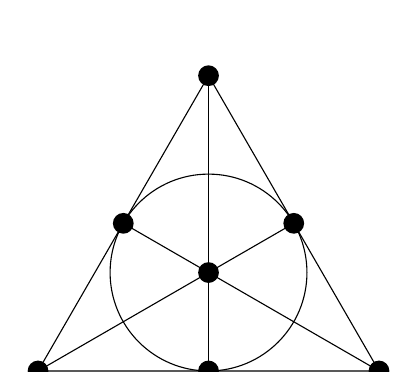
\begin{tikzpicture}[scale=2.5]

   \draw (0,0) circle (0.5);
   \draw (90:1) -- (-30:1)--(210:1)--cycle;

   \draw (90:1)--(0,0);
   \draw (210:1)--(0,0);
   \draw (-30:1)--(0,0);

   \draw (30:0.5)--(0,0);
   \draw (150:0.5)--(0,0);
   \draw (270:0.5)--(0,0);

   \fill (-0.866,-0.5) circle (1.5pt);
   \fill (0.866,-0.5) circle (1.5pt);
   \fill (0,-0.5) circle (1.5pt);
   \fill (0,1) circle (1.5pt);
   \fill (0,0) circle (1.5pt);
   \fill (0.433,0.25) circle (1.5pt);
   \fill (-0.433,0.25) circle (1.5pt);

\end{tikzpicture}
\caption{Fano Plane S(2,3,7)} \label{fig:fplane}
\end{figure}
The Fano plane is the geometry associated with S(2,3,7). Seven lines partition the seven points, where each line contains exactly three points, and each pair of points uniquely designates a line.


Using the Assmus-Mattson theorem to find the designs corresponding to $\mathcal{G}_{24}$ will require several definitions.
\begin{defn}[Dual Code and Totally Singular Code]
Suppose $\mathcal{C}$ is a linear code in vector space $V$. We denote 
$$\mathcal{C}^* = \{ \bm{u} \in V | \bm{u} \cdot \bm{w} = 0 \; \forall \; \bm{w} \in V \}. $$
If $\mathcal{C}$ is an $[n,k]$ code, then $\mathcal{C}^*$ is an $[n,n-k]$ code.
Furthermore, if $\mathcal{C}\subseteq\mathcal{C}^*$ then we call $\mathcal{C}$ \textit{totally singular}.
\end{defn}
We note that $\mathcal{G}_{24}$ is totally singular, because the rows of its generator matrix are orthogonal.
More explicitely $\bm{r}_i \cdot \bm{r}_j$ = 0 for any two rows in the matrix $\bm{A}$ of the generator matrix $[\bm{I}_{12}:\bm{A}]$ above. This implies $\mathcal{G}_{24} \subseteq \mathcal{G}_{24}^*$.
\begin{defn}[Self-dual]
If $\mathcal{C}$ is totally singular and $dim(\mathcal{C})=\frac{dim(V)}{2}$ then we can $\mathcal{C}$ is \textit{self-dual}.
\end{defn}
We just showed that $\mathcal{G}_{24}$ is totally singular, and we already know that $dim(\mathcal{G}_{24}) = 12 = \frac{24}/2$, so $\mathcal{G}_{24}$ is self-dual.
%\begin{defn}[We might not need this definition]
%A code $\mathcal{C}$ is \textit{double-even} if for every $x\in \mathcal{C}$, the weight of $c$ is divisible by 4.
%\end{defn}
\begin{thm}[Assmus-Mattson]
Let $\mathcal{C}$ be an $[n,k,d]$ binary code, and let $0<t<d$. Let $B_i$ be the number of vectors of weight $i$ in $\mathcal{C}^*$, and let
$$
s = |{i|B_i \not= 0 \; \& \; 0<i\leq n-t}|.
$$
If $s\leq d-t$, then the vectors of weight $d$ in $\mathcal{C}$ hold a t-design and the vectors of any weight $i\leq n-t$ and $B_i\not=0$ hold a t-design.
\end{thm}

Which naturally leads into the question we have been pursuing.
\begin{prop}
The $[24,12,8]_2$ code $\mathcal{G}_{24}$ is $S(5,8,24)$.
\end{prop}
\begin{proof} 
Since, all vectors in $\mathcal{G}_{24}$ are of weight 8, 12, or 16, we know that $s=3 \leq 8-5$. So the weight 8 words contain a 5-design [\cite{pless}]. More specifically we know that the minimum distance of the code is 8 and we can correct 3 errors, so 5 digits define a unique codeword, which demonstrates that the 5-design is in fact $S(5,8,24)$. This argument can also be applied to $\mathcal{G}_{23}$ to show that it corresponds to $S(4,7,23)$.
\end{proof}.

\section{Uniqueness of $\mathcal{G}_{24}$}
So far we have given two constructions of $\mathcal{G}_{23}$ and we have shown how to turn any construction of $\mathcal{G}_{23}$ into a construction of $\mathcal{G}_{24}$. Then we showed how we could consider $\mathcal{G}_{24}$ a Steiner system. We would like to say that the Golay codes are unique so that we can be sure that these constructions actually give us the same code. Again we will focus on $\mathcal{G}_{24}$ though our results will apply equally to $\mathcal{G}_{23}$. We will also use for free the uniqueness of the Steiner systems corresponding to our codes. What that leaves us to show, is that the code itself is unique and that no other code can correspond to $S(5,8,24)$.

\begin{thm}[Uniqueness of $\mathcal{G}_{24}$]
 The $[24,12,8]_2$ code $\mathcal{C}$ is unique.
\end{thm}

\begin{proof}
We will follow the proof given by Vera Pless in [\cite{pless}]. We want show that five coordinates specify a unique weight 8 codeword. We will first consider $\mathcal{C}$ punctured in some coordinate which we will label $\infty$ such that we preserve the dimension of the code. We call the resulting code $\mathcal{C}^{'}$ which has parameters $[23,12,7]_2$ or $[23,12,8]_2$. We showed that $[23,12,7]_2$ is perfect while $[23,12,8]_2$ is not, thus we argue $\mathcal{C}^{'}$ must be $[23,12,7]_2$ because $[23,12,8]_2$ does not partition the space. Consequently, we know that $[23,12,7]_2$ contains $S(4,7,23)$.
Now consider a set $S$ of five points containing $\infty$. Without $\infty$ this specifies a block in $S(4,7,23$ with weight 7. Because $\mathcal{C}$ has minimum weight 8, we know that the coordinate occupied by $\inf$ must be a 1 so that in $\mathcal{C}$ the weight is 8 and is contained in a unique block in $S(5,8,24)$.
Next consider a set $S$ of five points which does not include $\inf$. Then it exists in a unique sphere of radius centered at a codeword $\textbf{w}$ of weight 7 or a codeword $\textbf{v}$ of weight 8 in $\mathcal{C}$. From the previous argument $\textbf{v}$ must have a 1 at $\infty$. If $\textbf{w}$ has a 0 at $\inf$ then $S$ is contained in a a unique weight 8 set in $C$. If $\textbf{w}$ has a 1 at $\infty$, then pick four other points in $\mathbf{w}$. These five points are contained in a weight 8 set $\textbf{x}$ in $\mathcal{C}$ by the 4-design in $\mathcal{C}^{'}$. Then $weight(\textbf{x} + \textbf{w}) \leq 7$ which contradicts the minimum weight of $[24,12,8]_2$ being 8. Thus $\textbf{w}$ must contain a 5-design corresponding to $(5,8,24)$ which is unique by assumption.
\end{proof}

This is encouraging because we can be sure that all the constructions we have given of $\mathcal{G}_{24}$ actually produce the same code. The technique of puncturing a code and adding a point of infinite is a nice technique which will aid us in understanding the automorphism group of $\mathcal{G}_{24}$.

\section{The Automorphism Group of $\mathcal{G}_{24}$, $M_{24}$}
Knowing that $\mathcal{G}_{24}$ corresponds to the geometry of $S(5,8,24)$ work done by Witt showed that the automorphism group of $\mathcal{G}_{24}$ is $M_{24}$, the automorphism group of $S(5,8,24)$. We will only briefly touch on the basic definition and properties of $M_{24}$. For our purposes it is historically interesting as these relationships were exploited by Conway when classifying his three sporadic groups.
\begin{defn}[k-fold transitivity]
Let $G$ be a group acting on a set $S$, and $k \leq |S|$. We say that $G$ is k-fold transitive on $S$ if, given any two ordered k-tuples $(x_1, \ldots , x_k)$ and $(y_1, \ldots, y_k)$ of elements in $S$, there is an element $g \in G$ such that $x_i g = y_i$ for all $i \in 1,\ldots , k$, if such a $g \in G$ is unique, then we call $G$ sharply k-fold transitive on $S$.
\end{defn}
\begin{defn}[Mathieu Group $M_{24}$]
The sporadic group $M_{24}$ is the automorphism group of $S(5,8,24)$ generated by
\begin{enumerate}
\item $\alpha = (\infty)(0 \: 1 \: 2 \: \ldots \: 22)$
\item $\gamma = (0 \: \infty)(1 \: 22)(2 \: 11)(3 \: 15)(4 \: 17)(5 \: 9)(6 \: 19)(7 \: 13)(8 \: 20)(10 \: 16)(12 \: 21)(14 \: 18)$
\item $\beta = (\infty)(0)(3)(15)(1 \: 18 \: 4 \: 2 \: 6)(5 \: 21 \: 20 \: 10 \: 7)(8 \: 16 \: 13 \: 9 \: 12)(11 \: 19 \: 22 \: 14 \: 17).$
\end{enumerate}
$M_{24}$ operates 5-fold transitively on $S(5,8,24)$ [\cite{conway}].
\end{defn}

\begin{thm}[The order of $M_{24}$]
The order of $M_{24}$ is $759 \cdot 16 \cdot 20160.$
\end{thm}

We will provide a extremely truncated sketch of the proof.
\begin{proof}
Let $\Omega = \{0, \: 1, \: \ldots, \: 22, \: \infty \}$, $F$ the subgroup of $M_{24}$ which permutes $\{ a_1, \ldots , a_8 \}$ and $H$ be the subgroup of $F$ that fixes $a_9$ of $\Omega$. Then we can show that $[M_{24} : F] = 759$, $|H| = |A_8| = 20160$, $[F:H] = 16$, therefore $|M_{24}| = 759 \cdot 16 \cdot 20160 = 244,823,040.$
\end{proof}

While $M_{24}$ is the automorphism group of $\mathcal{G}_{24}$, the other Mathieu groups are stabilizers of subsets of $\mathcal{G}_{24}$. Where $M_{23}$ stabilizes a single coordinate, $M_{22}$ stabilizes a pair of coordinates, $M_{12}$ stabilizes a codewords of weight 12, and $M_{11}$ stabilizes a codeword of weight 12 and one other coordinate [$find \; reference$]. All together these groups are subgroups of Conway's simple sporadic groups, and ultimately the Monster group.

\section{conclusion}
So we see how Golay's half page article has had ramifications throughout mathematics, making connection to combinatorics, geometry, algebra, and helping establish coding theory as an independent field. Outside of mathematics Golay's code has carried pictures taken from outside of our solar system, 40 billion miles away. Pictures containing enough information to detect Earth as a blue speck using less than a full pixel's worth of information.
\clearpage
\printbibliography
%----------------------------------------------------------------------------------------

\end{document}